%\documentclass[a4paper]{scrartcl}
\documentclass[a4paper]{article}
\usepackage{setspace}
\usepackage{url}
\usepackage{mdwlist}
\usepackage{polski}
\usepackage[utf8x]{inputenc}
\usepackage{color}
\usepackage{mathtools}
\usepackage{graphicx}
\usepackage[unicode=true]{hyperref}
\usepackage{multirow}
\usepackage[table]{xcolor}
\usepackage{subfig}
\usepackage{listings}
\usepackage[backgroundcolor=white]{todonotes}
\definecolor{dkgreen}{rgb}{0.2,0.8,0.2}
\definecolor{gray}{rgb}{0.5,0.5,0.5}
\definecolor{mauve}{rgb}{0.58,0,0.82}
\newcommand{\HRule}{\rule{\linewidth}{0.5mm}}
\newcommand{\siatkonator}{\textbf{Siatkonator} }
\renewcommand{\triangle}{\href{http://www.cs.cmu.edu/~quake/triangle.html}{triangle}}
\lstset{ %
  basicstyle=\ttfamily\footnotesize,
  numbers=left,
  numberstyle=\footnotesize,
  stepnumber=1,
  numbersep=5pt,
  breaklines=true,
  tabsize=2,
  showspaces=false,
  showstringspaces=false,
  frame=single,
  numberstyle=\tiny\color{gray},
  keywordstyle=\color{mauve},
  commentstyle=\color{dkgreen},
  stringstyle=\color{mauve},
}

\begin{document}
\begin{titlepage}

  \begin{center}


    % Upper part of the page
    
\includegraphics[width=0.3\textwidth]{logo.jpg}\\[1cm]

    \begin{onehalfspace}
      \textsc{\LARGE Wydział Elektryczny Politechniki Warszawskiej}\\[1.5cm]
    \end{onehalfspace}



    \textsc{Języki i~Metody Programowania II -- projekt 1}\\[0.5cm]

    % Title
    \HRule \\[0.4cm]
    {\huge \bfseries Siatkonator }\\[0.2cm]
    \HRule \\[1.5cm]

    % Author and supervisor
    \begin{flushleft} \large
      \emph{Autor:}\\
      Barnaba \textsc{Turek}\\
      \href{mailto:barnabaturek@gmail.com}{barnabaturek@gmail.com}
    \end{flushleft}
    \vfill

    % Bottom of the page
    {\large \today}

  \end{center}

\end{titlepage}
\sloppy

\setcounter{tocdepth}{4}
\tableofcontents

\section{Specyfikacja funkcjonalna}
\subsection{Program}
\siatkonator to program sklejający siatki trójkątne.
Program przyjmuje jedną lub więcej siatek trójkątnych oraz jeden wielokąt.

Wynikiem działania programu jest siatka trójkątna opisująca zadany wielokąt, która zawiera podane określone siatki.

\begin{figure}[h]
  \centering
  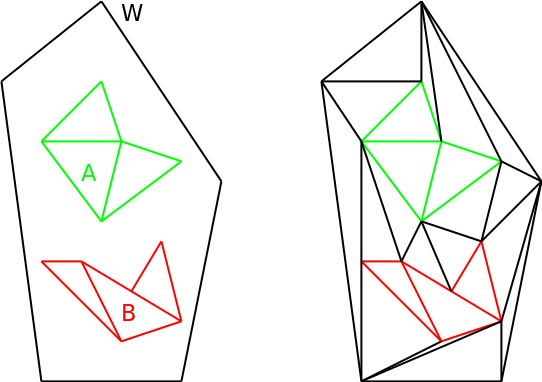
\includegraphics[width=0.5\textwidth]{ilustracja.png}
  \caption{przykład sklejania zadanego wielokątu W~i~siatek A~i~B}
\end{figure}

\subsection{Wywołanie}
Program nie prowadzi dialogu z~użytkownikiem.

\begin{lstlisting}[caption=Przykładowe wywołanie]
  $ siatkonator -e siatka1.ele -e siatka2.ele polygon.poly
\end{lstlisting}

Ostatni argument programu określa nazwę pliku (wraz ze ścieżką) w~którym opisany jest wielokąt.
Nie podanie tego argumentu spowoduje błąd wykonania programu.

Wcześniejsze argumenty określają opcje wykonania programu i~nie są wymagane.
Kolejność argumentów nie ma znaczenia.

Dostępne są następujące opcje:
\begin{description}
  \item[\texttt{-e <name>}] dodaje siatkę, która zostanie ``sklejona'' z~wielokątem. Program zakłada, że istnieje także plik o~takiej samej nazwie bazowej z~rozszerzeniem \texttt{node} opisujący wierzchołki.
  \item[\texttt{-o <name>}] podaje nazwę pliku wyjściowego. W~przypadku braku tego parametru wynik zostanie wypisany na standardowe wejście (najpierw plik ele, potem node).
  \item[\texttt{-a <area>}] określa maksymalną powierzchnię trójkąta (nie zmienia zadanych siatek!).
  \item[\texttt{-q <degrees>}] określa minimalną miarę kąta w~trójkącie w~wygenerowanej siatce trójkątnej (nie zmienia zadanych siatek!),
\end{description}

W~przypadku powodzenia program zwraca zero. W~przeciwnym wypadku program zwraca jeden z~kodów błędu:

\begin{description}
  \item[\texttt{kod 1}] Błąd otwarcia pliku (spowodowany np. brakiem uprawnień lub pliku).
  \item[\texttt{kod 2}] Błąd wczytania pliku (spowodowany błędnym formatem któregoś z~plików źródłowych).
  \item[\texttt{kod 3}] Błędny format argumentów linii poleceń.
\end{description}

Ponadto program w~czasie działania wypisuje informacje o~swoim aktualnym stanie na wyjście \texttt{STDERR}.

\subsection{Pliki}
\siatkonator korzysta z~plików w~formatach \texttt{poly}, \texttt{ele} i~\texttt{node}.

\begin{description}
  \item[poly] \href{http://www.cs.cmu.edu/~quake/triangle.poly.html}{format pliku opisującego wielokąt}
  \item[ele] \href{http://www.cs.cmu.edu/~quake/triangle.ele.html}{format pliku opisującego z~których wierzchołków składają się trójkąty siatki}
  \item[poly] \href{http://www.cs.cmu.edu/~quake/triangle.poly.html}{format pliku opisującego wierzchołki siatki}
\end{description}

Wszystkie wykorzystywane formaty są zgodne z~formatami wykorzystywanymi przez program \triangle.

\subsection{Dodatkowe uwagi}
Odradzam użytkownikowi podawanie programowi siatek, które przecinają się ze sobą, bądź przecinają się z~podanym wielokątem.
Jeżeli użytkownik koniecznie chce podać bezsensowne dane, to otrzyma bezsensowne wyniki.
Taka sytuacja nie jest rozumiana jako błąd programu i~nie jest do niej przypisany żaden kod błędu.

\newpage
\section{Specyfikacja implementacyjna}
\subsection{Struktura programu}

\begin{figure}[h]
  \centering
  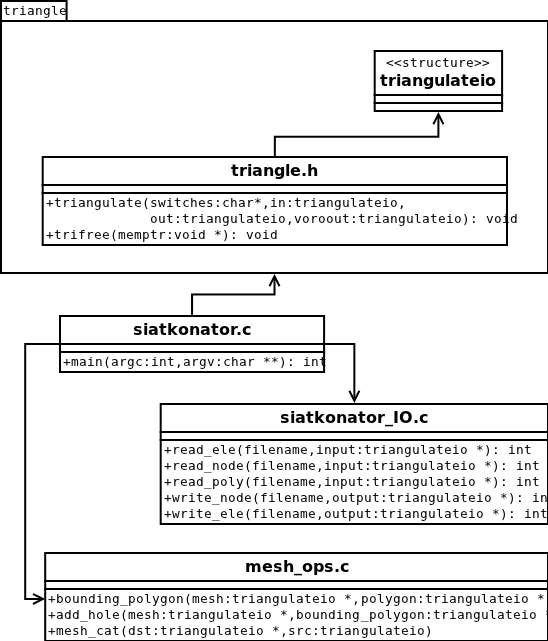
\includegraphics[width=0.8\textwidth]{class.png}
  \caption{Diagram klas}
\end{figure}

  Program podzielony jest na trzy pliki:
  \begin{description}
    \item[siatkonator.c] Plik zawierający główną funkcję odpowiedzialną za wczytanie argumentów i~zależnie od nich wykonanie algorytmu sklejania siatek.
    \item[siatkonator\_IO.c] Plik zawierający funkcje związane z~czytaniem i~zapisywaniem plików \emph{node}, \emph{ele} i \emph{poly} do struktur \texttt{triangulateio}.
    \item[mesh\_ops.c] Plik zawierający funkcje obsługujące logikę sklejania siatek (znajdowanie wielokąta otaczającego siatkę, wycinanie dziur w~siatkach i~łączenie siatek).
    \item[common.c] Plik zawierający funkcje pomocnicze (takie jak wypisywanie wiadomości).
  \end{description}

\subsubsection{Funkcje modułu \texttt{mesh\_ops}}
\begin{description}
  \item[\texttt{bounding\_polygon}] funkcja przyjmująca wskaźnik na wczytaną gotową siatkę i~znajdująca otaczający ją wielokąt (który należy wyciąć z~otoczki przed przeprowadzeniem triangulacji).
  \item[\texttt{add\_hole}] Funkcja przyjmująca wskaźnik na wczytaną otoczkę (być może już z~dziurami) i~na wielokąt otaczający jedną ze sklejanych siatek. Funkcja dodaje do otoczki dziurę w~miejscu, w~którym zostanie w~nią wklejona siatka.
  \item[\texttt{mesh\_cat}] Funkcja przyjmująca dwa wskaźniki na siatki i~dodająca elementy drugiej siatki do elementów pierwszej siatki.
\end{description}

\subsection{Algorytmy}
\begin{lstlisting}[caption=Pseudokod algorytmu głównej funkcji programu sklejającej siatki]
  wczytaj dane z pliku poly do struktury p
  dla kazdego pliku .ele:
    wczytaj dane z plikow ele i nodes do struktury E
    znajdz w strukturze E krawedzie, ktore wystepuja tylko raz
    usun te krawedzie ze struktury E
    dodaj te krawedzie do struktury P jako sekcje
    dodaj dziure do struktury P wewnatrz kazdego trojkata ze struktury E
  wykonaj triangulacje na strukturze p do siatki S
  dla kazdego pliku .ele:
    wstaw siatke z pliku do dziur w siatce S
  zapisz wynik triangulacji do plikow ele i node
\end{lstlisting}

\begin{lstlisting}[caption=Pseudokod funkcji szukającej wielokąta otaczającego daną siatkę: \texttt{bounding\_polygon}]
  H - tablica mieszajaca

  Dla kazdego wierzcholka w:
    jezeli H[w] istnieje:
      Dodaj w do H
    else:
      Usun w z~H

  Dla kazdego wierzcholka w:
    jezeli H[w] istnieje:
      dodaj w~do wielokata otaczajacego
      usun w~z~wielokata otaczajacego

  Dodaj dziure w~wielokacie otaczajacym w~miejscu srodka ciezkosci pierwszego elemenetu.

\end{lstlisting}

\subsection{struktury danych}
Struktura danych, której będę używał do komunikacji między funkcjami to struktura \texttt{triangulateio} dostarczona wraz z~programem triangle.
Struktura ta pozwala opisać siatkę na każdym etapie jej budowania (także siatki wyjściowe).

Jej wadą jest fakt, że nie jest specjalizowana do konkretnych zadań i~wiele pól nie będzie miało zastosowania.
Mimo to jest już napisana, udokumentowana i~mogę być pewien, że zawiera wszystkie potrzebne pola.

Zastosowanie innej struktury, jako struktury pośredniej wymagałoby tłumaczenia jej do \texttt{triangulateio} przed wykonaniem funkcji \texttt{triangulate()}.

\subsection{Rozwiązywanie konfliktów atrybutów wierzchołków}
Program bierze pod uwagę tylko pierwszy atrybut każdego wierzchołka.

Wczytując pliki program zapamiętuje najniższy i~najwyższy atrybut wierzchołka w~danym pliku.
Następnie program oblicza stałą, o~którą należy przesunąć atrybuty wierzchołka w~tym pliku, aby nuniknąć konfliktu.

\begin{lstlisting}[caption=Przykład]
  Jezeli w~pliku A.poly atrybuty wierzcholkow sa z~zakresu 1..10,
  I~w~pliku B.node atrybuty sa z~zakresu 3..10,
  To po wczytaniu A.poly najwiekszy znaleziony atrybut jest 10,
  I~po wczytaniu B.node najmniejszy znaleziony atrybut bedzie 3,
  Wiec nalezy wszystkie atrybuty wierzcholkow znalezionych w~B.node przesunac o~(10-3)
\end{lstlisting}

W~związku z~tym wynik działania programu \textbf{zależy} od kolejności podanych plików wejściowych.

Po takim podziale pozostała przestrzeń zmiennej używana jest do rozwiązywania konfliktów wynikających z~tego, że dwa wierzchołki o~różnych atrybutach znalazły się w~tym samym miejscu.

Jeśli oba wierzchołki mają taką samą wartość atrybutu, atrybut \textbf{nie zostaje} zachowany (wynika to z~faktu rozdzielenia przestrzeni atrybutów).

Jeśli oba wierzchołki mają różną wartość atrybutów, zostaje im przydzielona nowa wartość z~zakresu wartości przeznaczonego na konflikty za pomocą prostej funkcji mieszającej
(znajdowana jest największa liczba pierwsza w~dostępnym zakresie. Atrybut nowego wierzchołka to:

\begin{lstlisting}[caption=]
(Atrybut\ A + Atrybut\ B) % (liczba pierwsza) + offset zakresu
\end{lstlisting}

Takie rozwiązanie gwarantuje, że elementy będące połączeniem danych atrybutów zawsze będą miały ten sam atrybut w~pliku wynikowym.

\begin{figure}[h]
  \centering
  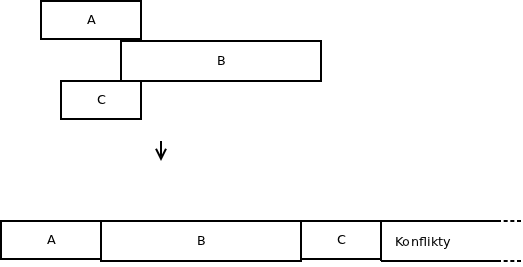
\includegraphics[width=0.8\textwidth]{konflikty.png}
  \caption{przykład podziału przestrzeni atrybutów}
\end{figure}





\end{document}
